\appendix
\chapter{Shrinking sphere centering method}
\label{app:shrinking_sphere}

This appendix gives the mathematical formulation and a direct algorithmic implementation of the shrinking-sphere centering routine used in the analysis.

Let the particle set be indexed by $i$, with positions $\mathbf{x}_i\in\mathbb{R}^3$ and masses $m_i>0$. Define the mass-weighted centroid over an index set $S$ as
\begin{equation}
\mathbf{C}(S) = \frac{\sum_{i\in S} m_i\,\mathbf{x}_i}{\sum_{i\in S} m_i}.
\end{equation}

Initialize
\begin{equation}
S_0 = \{1,\dots,N\},\qquad \mathbf{x}_0 = \mathbf{C}(S_0),\qquad R_0 = \max_{i\in S_0}\|\mathbf{x}_i-\mathbf{x}_0\|.
\end{equation}

For iterations $k=0,1,2,\dots$ define the restricted set and update rules
\begin{align}
S_{k+1} &= \{i\in S_k:\ \|\mathbf{x}_i-\mathbf{x}_k\| < R_k\}, \\
\mathbf{x}_{k+1} &= \mathbf{C}(S_{k+1}), \\
R_{k+1} &= f_s\,R_k,
\end{align}
with shrink factor $0<f_s<1$ (implementation default $f_s=0.9$).

Stop when either
\begin{equation}
\|\mathbf{x}_{k+1}-\mathbf{x}_k\| < \delta \quad\text{or}\quad |S_{k+1}| < N_{\min},
\end{equation}
and return $\mathbf{x}_{\mathrm{final}}=\mathbf{x}_{k+1}$. Typical choices used in the analysis are $\delta=10^{-5}$ (code length units) and $N_{\min}=100$.

The same logic can be written in compact pseudocode as follows:
\begin{lstlisting}[basicstyle=\footnotesize\ttfamily,breaklines=true]
function shrinking_sphere_center(pos[N,3], mass[N], f_s=0.9, delta=1e-5, N_min=100):
	x = weighted_average(pos, mass)
	R = max(norm(pos - x, axis=1))
	while True:
		r = norm(pos - x, axis=1)
		mask = (r < R)
		if mask.sum() < N_min:
			break
		x_new = weighted_average(pos[mask], mass[mask])
		if norm(x_new - x) < delta:
			x = x_new
			break
		x = x_new
		R = R * f_s
	return x
\end{lstlisting}


\appendix
\chapter{Shells}


\subsection{Analytic shell decomposition}

Following the framework established in Chapter 3, the halo is decomposed into logarithmically spaced shells and the exact analytic contributions of each shell to the gravitational potential and force are computed. The key physical insight is the shell theorem: in a spherically symmetric system, outer shells contribute to the potential everywhere inside them, but only the enclosed mass contributes to the radial force.

For an NFW profile with parameters $\rho_s = 10^7 \, M_{\odot}/\mathrm{kpc}^3$, $r_s = 10 \, \mathrm{kpc}$, $r_{\mathrm{vir}} = 100 \, \mathrm{kpc}$, the analysis computes: (i) the enclosed mass $M(<r)$ and shell mass distribution, (ii) the contribution of each shell to the potential depth at the center, (iii) the fraction of potential at arbitrary probe radii originating from material outside a chosen cutoff radius, and (iv) a 2D diagnostic map showing these fractions for all radius combinations.

\subsection{Mass and potential distribution across the halo}

The first two diagnostics establish the overall radial structure of the halo. Figure \ref{fig:results_shell_mass} shows the enclosed mass profile and the fractional mass distribution per shell.

\begin{figure}[H]
	\centering
	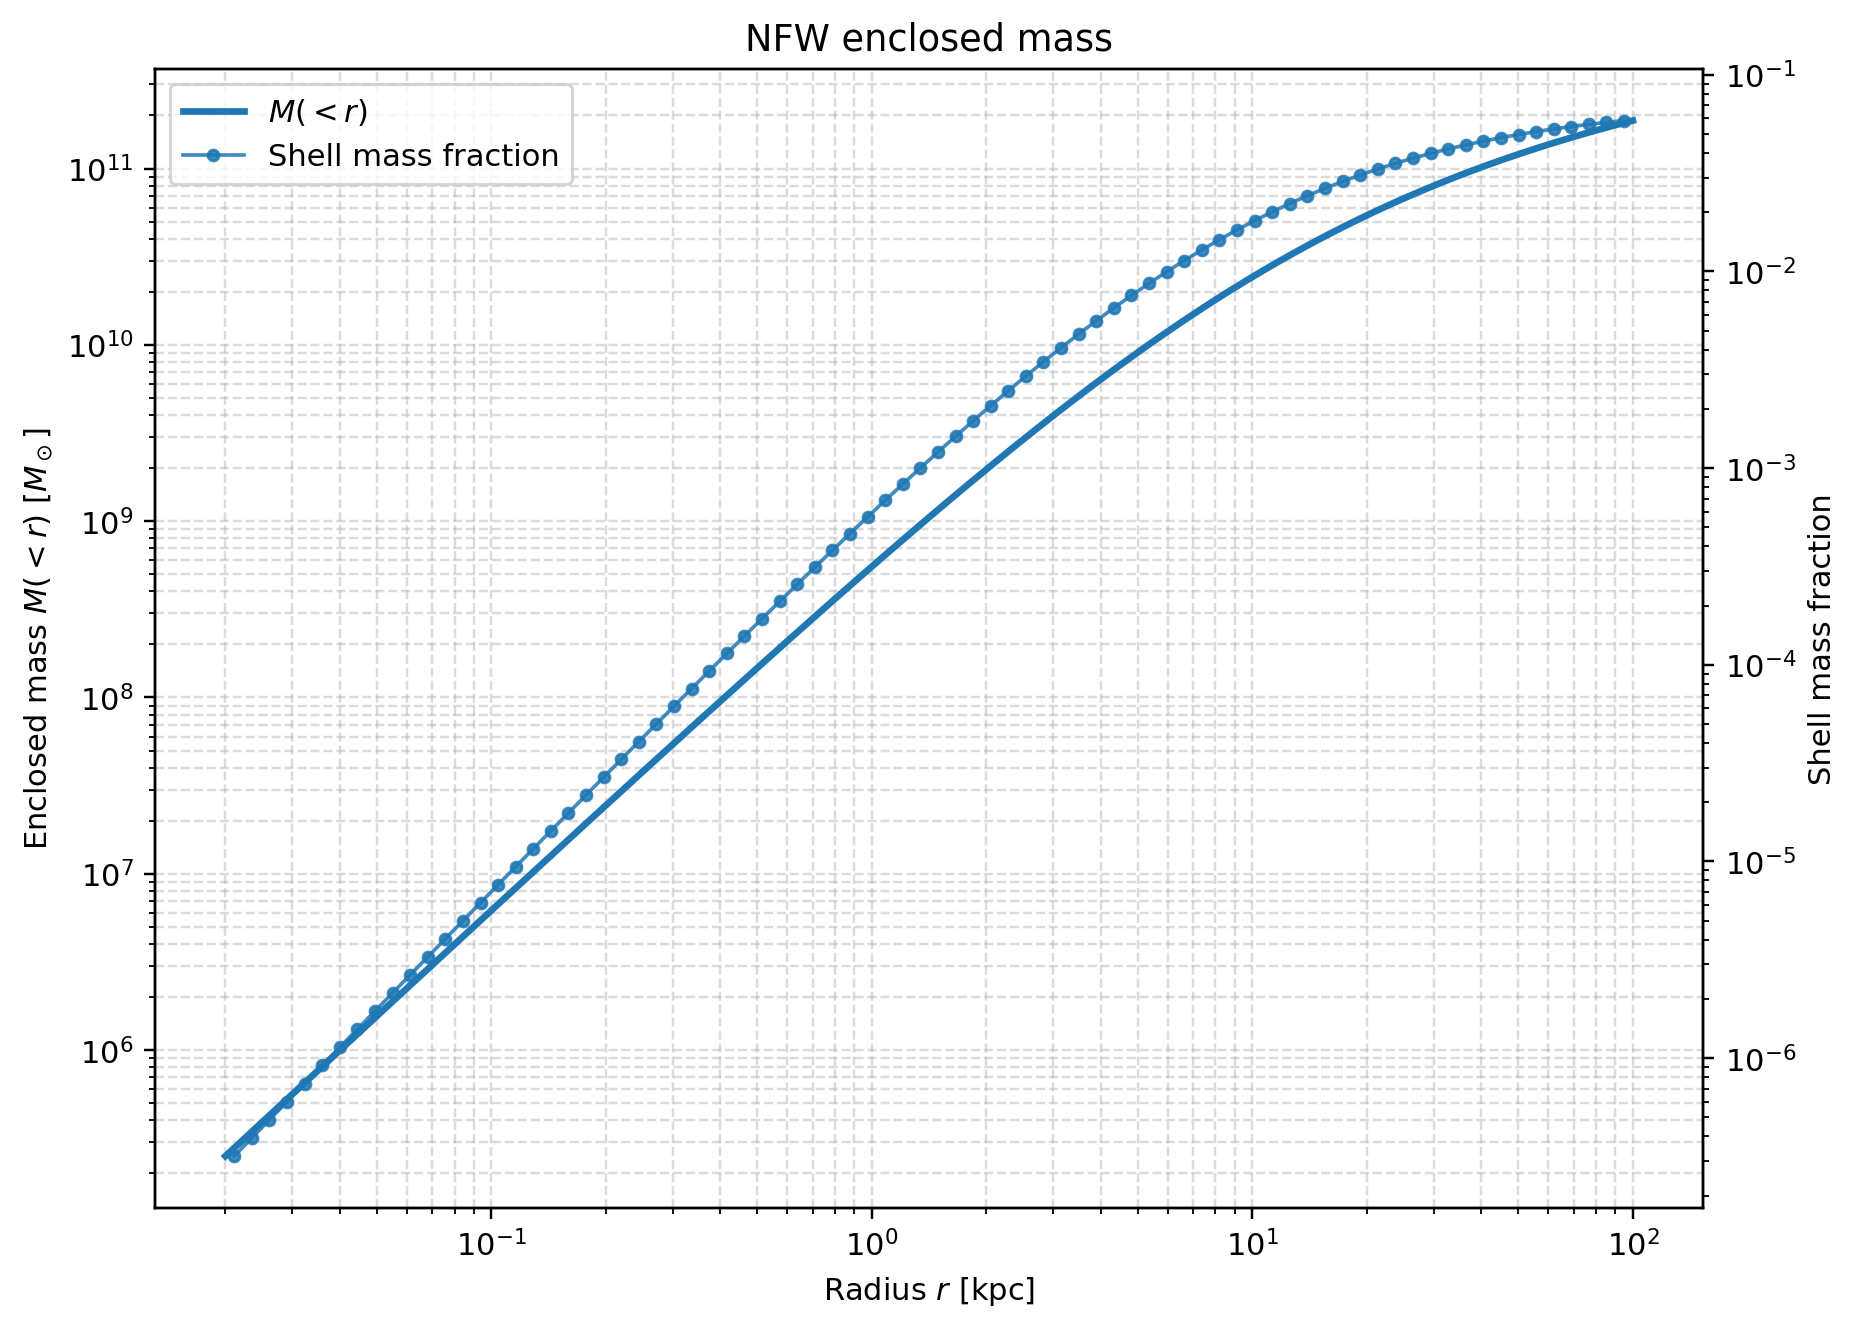
\includegraphics[width=0.85\textwidth]{content/ch5/img/01_mass_profile_and_shell_fraction.png}
	\caption{\textbf{NFW enclosed mass and shell mass fraction.} Left axis: monotonically increasing enclosed mass $M(<r)$ with radius. Right axis: shell mass fraction per logarithmic shell.}
	\label{fig:results_shell_mass}
\end{figure}

The enclosed-mass profile follows the expected NFW form: steep near the center and flattening at larger radii. Importantly, the shell mass fraction plot shows that although the inner shells contain many particles per unit volume (high density), the integrated mass grows progressively outward. Shells at radii $r > 20$ kpc contain a cumulatively significant mass fraction, establishing that the outer halo is not negligible.

Figure \ref{fig:results_shell_potential} shows the contribution of each shell to the gravitational potential at the center and the cumulative contribution from all shells outside a given radius.

\begin{figure}[H]
	\centering
	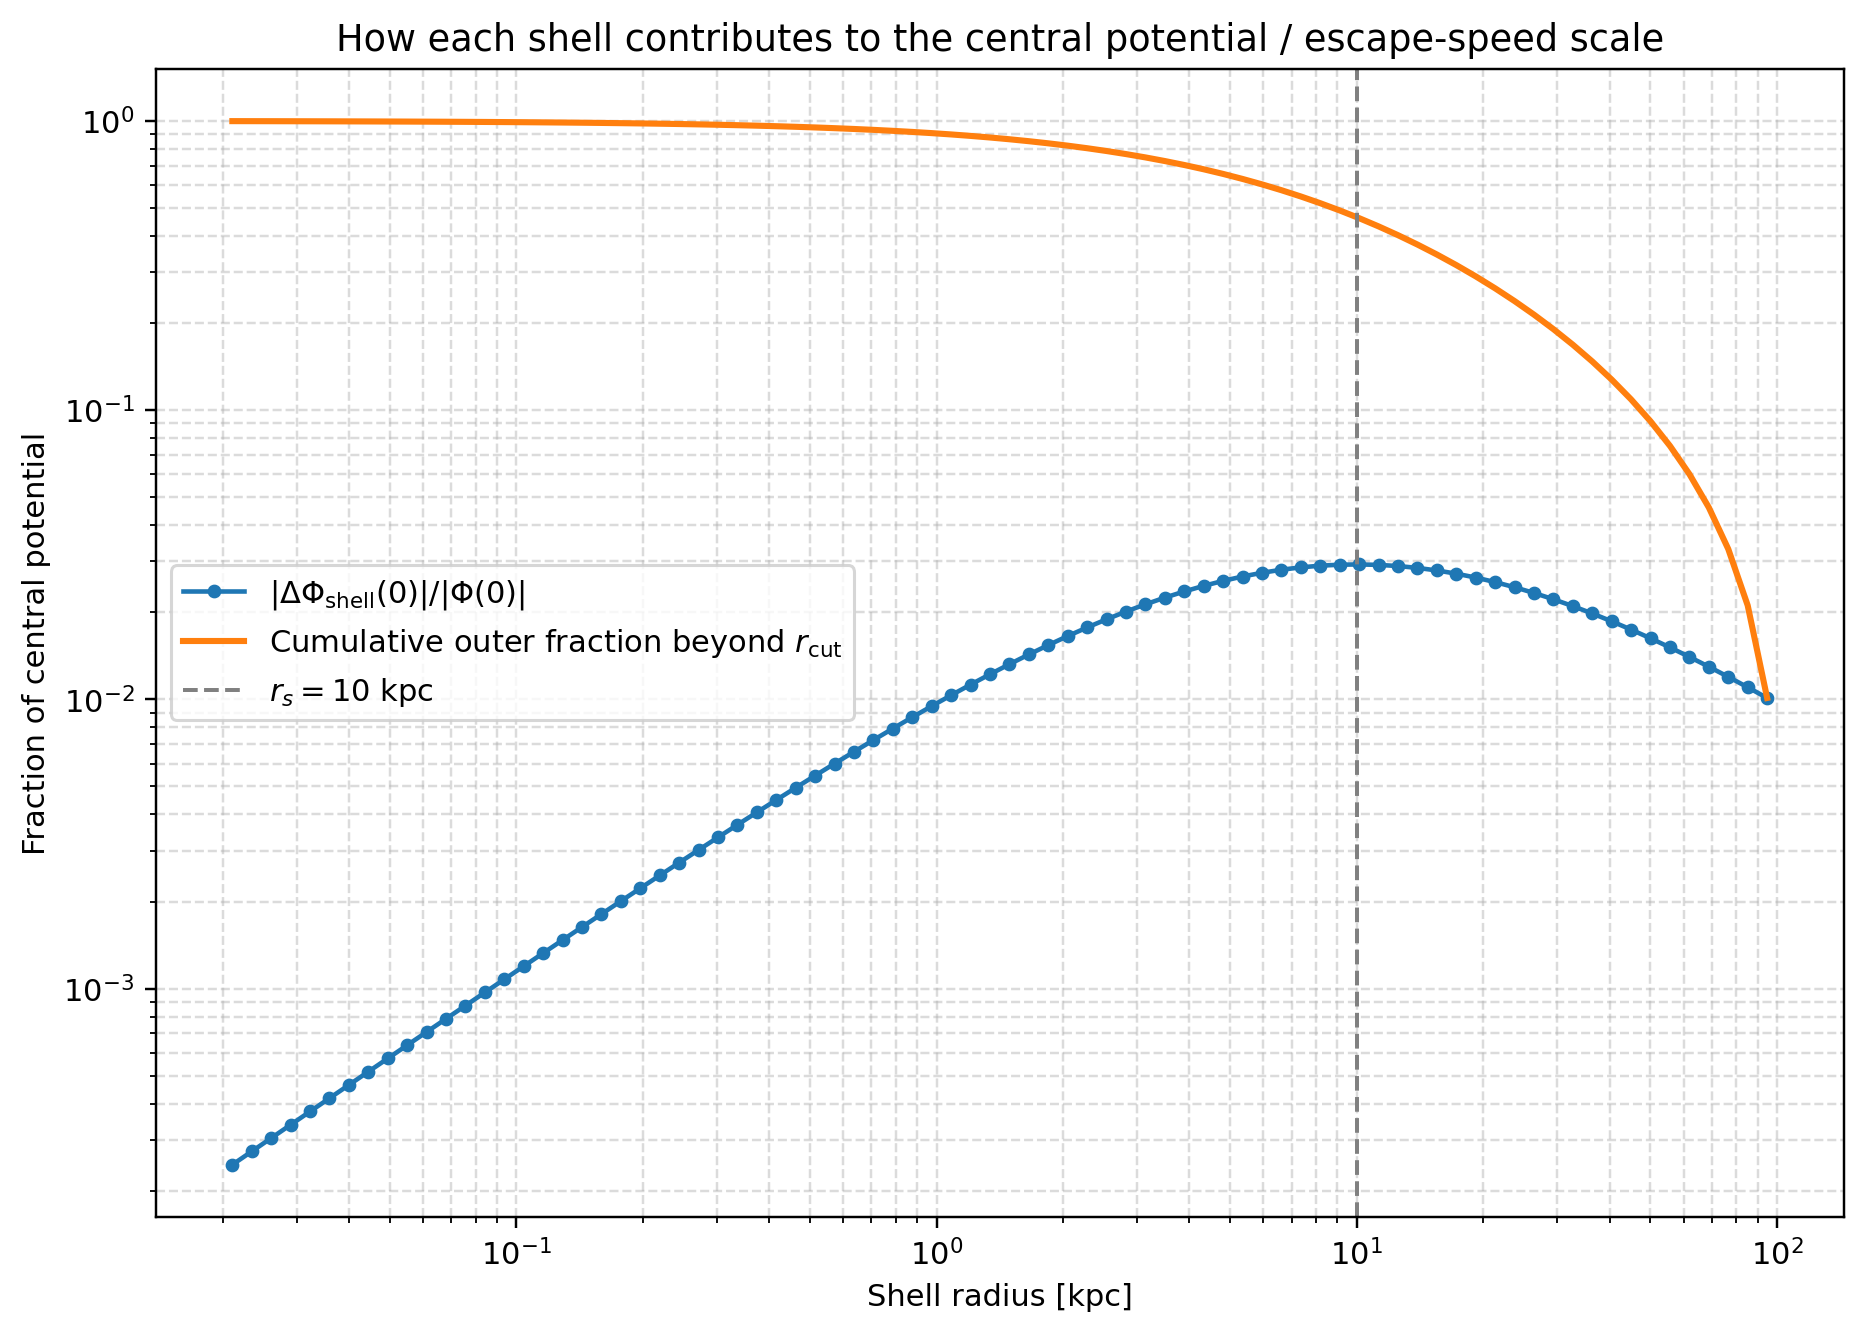
\includegraphics[width=0.85\textwidth]{content/ch5/img/02_central_potential_shell_contribution.png}
	\caption{\textbf{Shell contributions to the central potential depth.} Individual shells (blue points with error bars) contribute to the total potential depth $|\Phi(0)|$. The cumulative contribution (orange line) from all shells beyond a given radius shows that shells at radii beyond the scale radius $r_s$ still make substantial contributions to the escape-speed scale.}
	\label{fig:results_shell_potential}
\end{figure}

The key finding here is that shells well outside the center, at radii several times the scale radius, still contribute visibly to the potential depth. The fractional contribution decreases with radius but remains non-negligible up to $r \sim 3 r_s$. This result motivates the choice of cutoff radius in the hybrid model; setting $r_{\mathrm{cut}}$ too small would omit a significant part of the potential structure.

\subsection{Outer-halo influence as a function of cutoff radius}

The most critical diagnostic for the hybrid model design is the outer potential fraction. The fraction of the total potential at a given probe radius that arises from material beyond a chosen cutoff radius. Figure \ref{fig:results_shell_cutoff} shows this quantity for several probe radii as the cutoff radius is increased.

\begin{figure}[H]
	\centering
	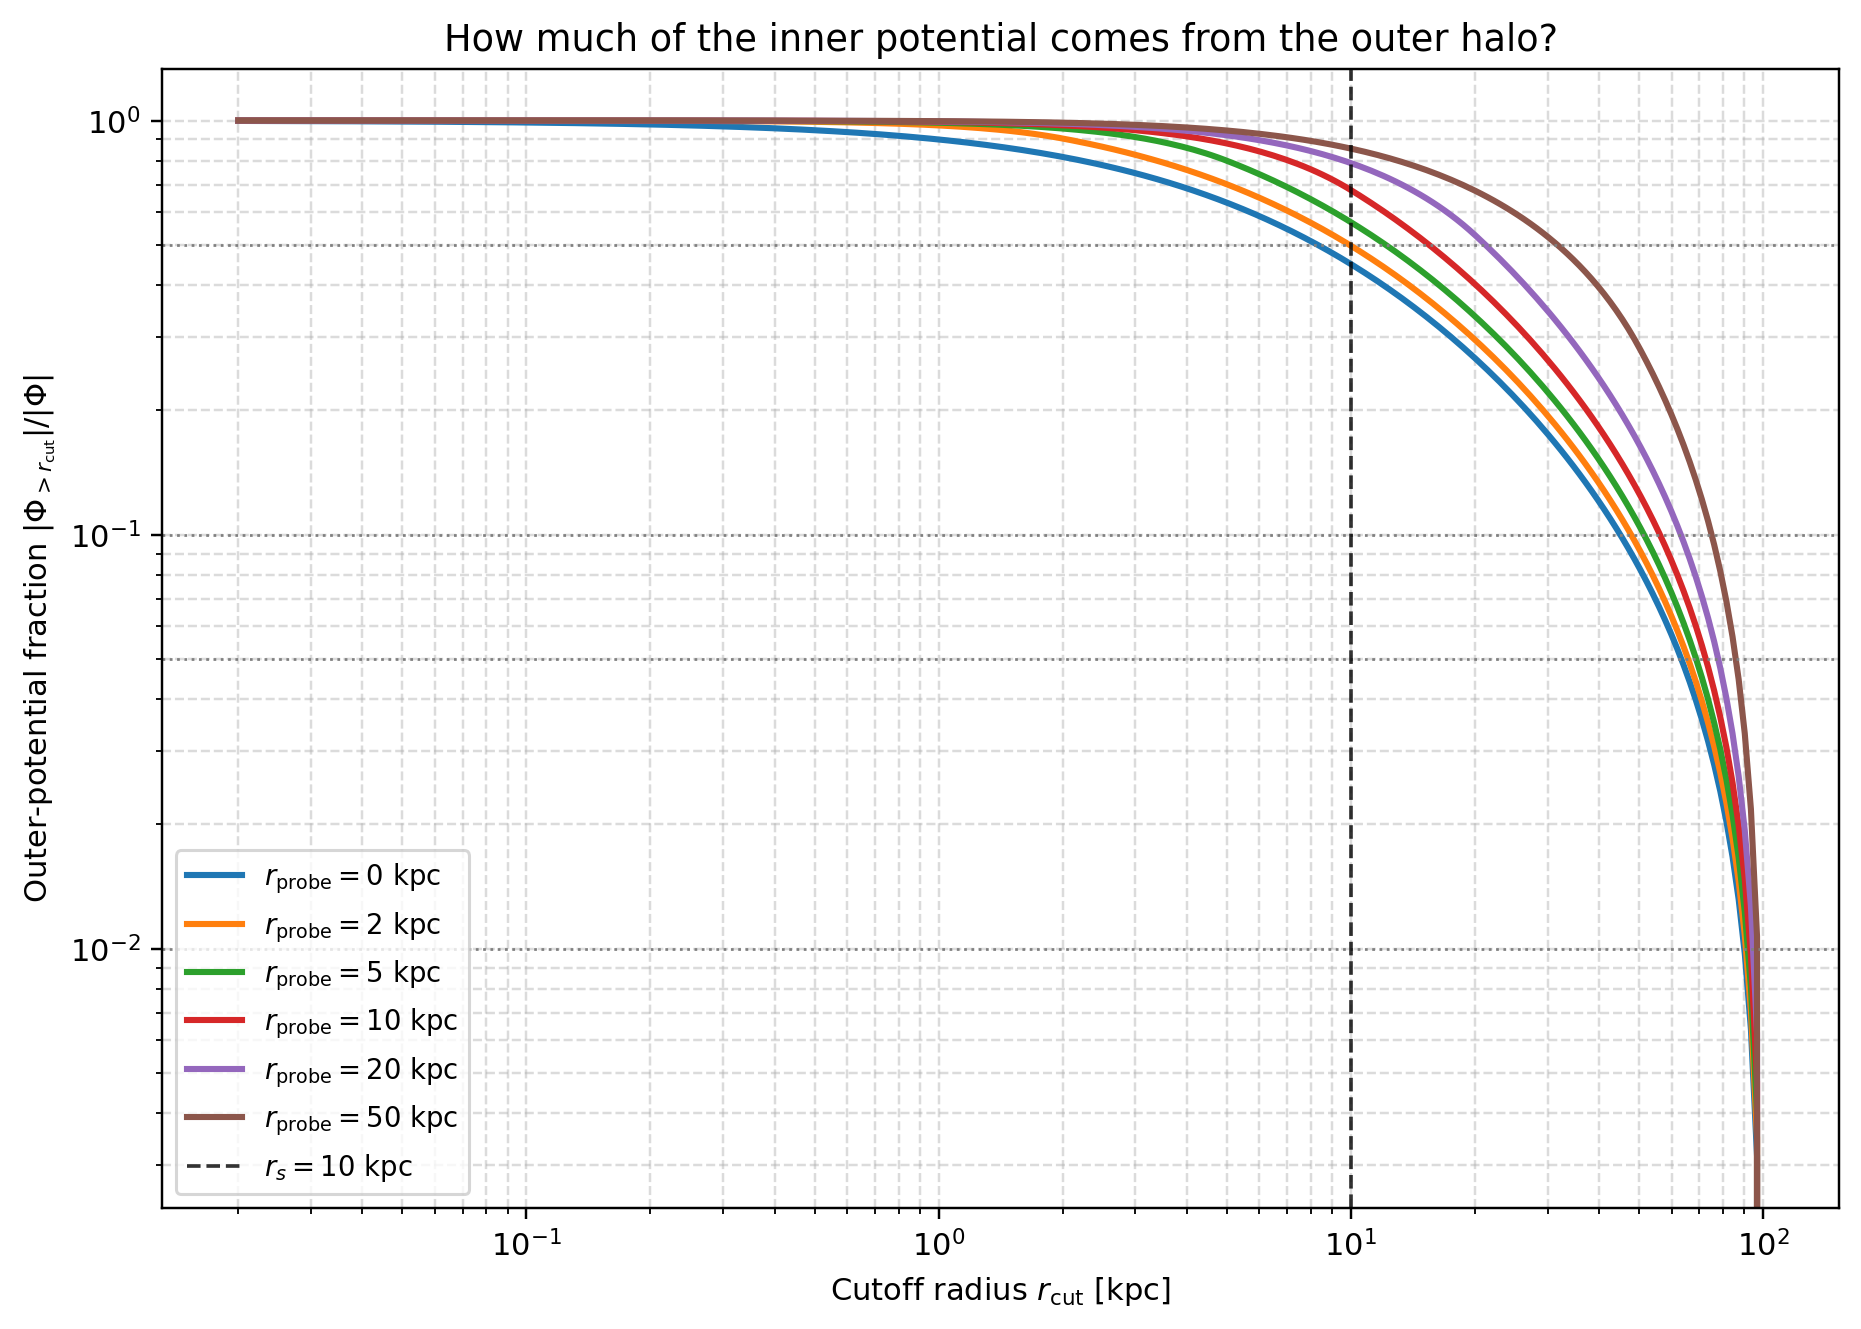
\includegraphics[width=0.85\textwidth]{content/ch5/img/03_outer_fraction_vs_cutoff.png}
	\caption{\textbf{Outer-potential fraction versus cutoff radius.} For probe radii ranging from the center to $r = 5 r_s$, the fraction of the potential originating from material beyond the cutoff radius $r_{\mathrm{cut}}$ is plotted against the cutoff. As the cutoff moves outward, the outer contribution drops sharply initially, then plateaus. For the central region ($r_{\mathrm{probe}} < r_s$), a cutoff at $r_{\mathrm{cut}} \approx 10$ kpc retains roughly 5--10\% of the potential from the outer halo; at $r_{\mathrm{cut}} \approx 30$ kpc, this drops below 1\%. Thus, if the outer halo contributes significantly to the potential at the radii of interest (e.g., $r < 1$ kpc for the central density), then the outer region must be represented accurately.}
	\label{fig:results_shell_cutoff}
\end{figure}

The curves in this figure answer the central question: how large must $r_{\mathrm{cut}}$ be to capture the essential potential structure? For the central region, a cutoff at $r_{\mathrm{cut}} = 10$ kpc retains the majority of the potential at small radii while excluding the outermost, kinematically less important material. This is a quantitative justification for the parameter choice in the numerical hybrid experiment.

\subsection{2D outer-fraction map}

Figure \ref{fig:results_shell_map} provides a compact summary of the outer-potential fraction across all combinations of probe and cutoff radii.

\begin{figure}[H]
	\centering
	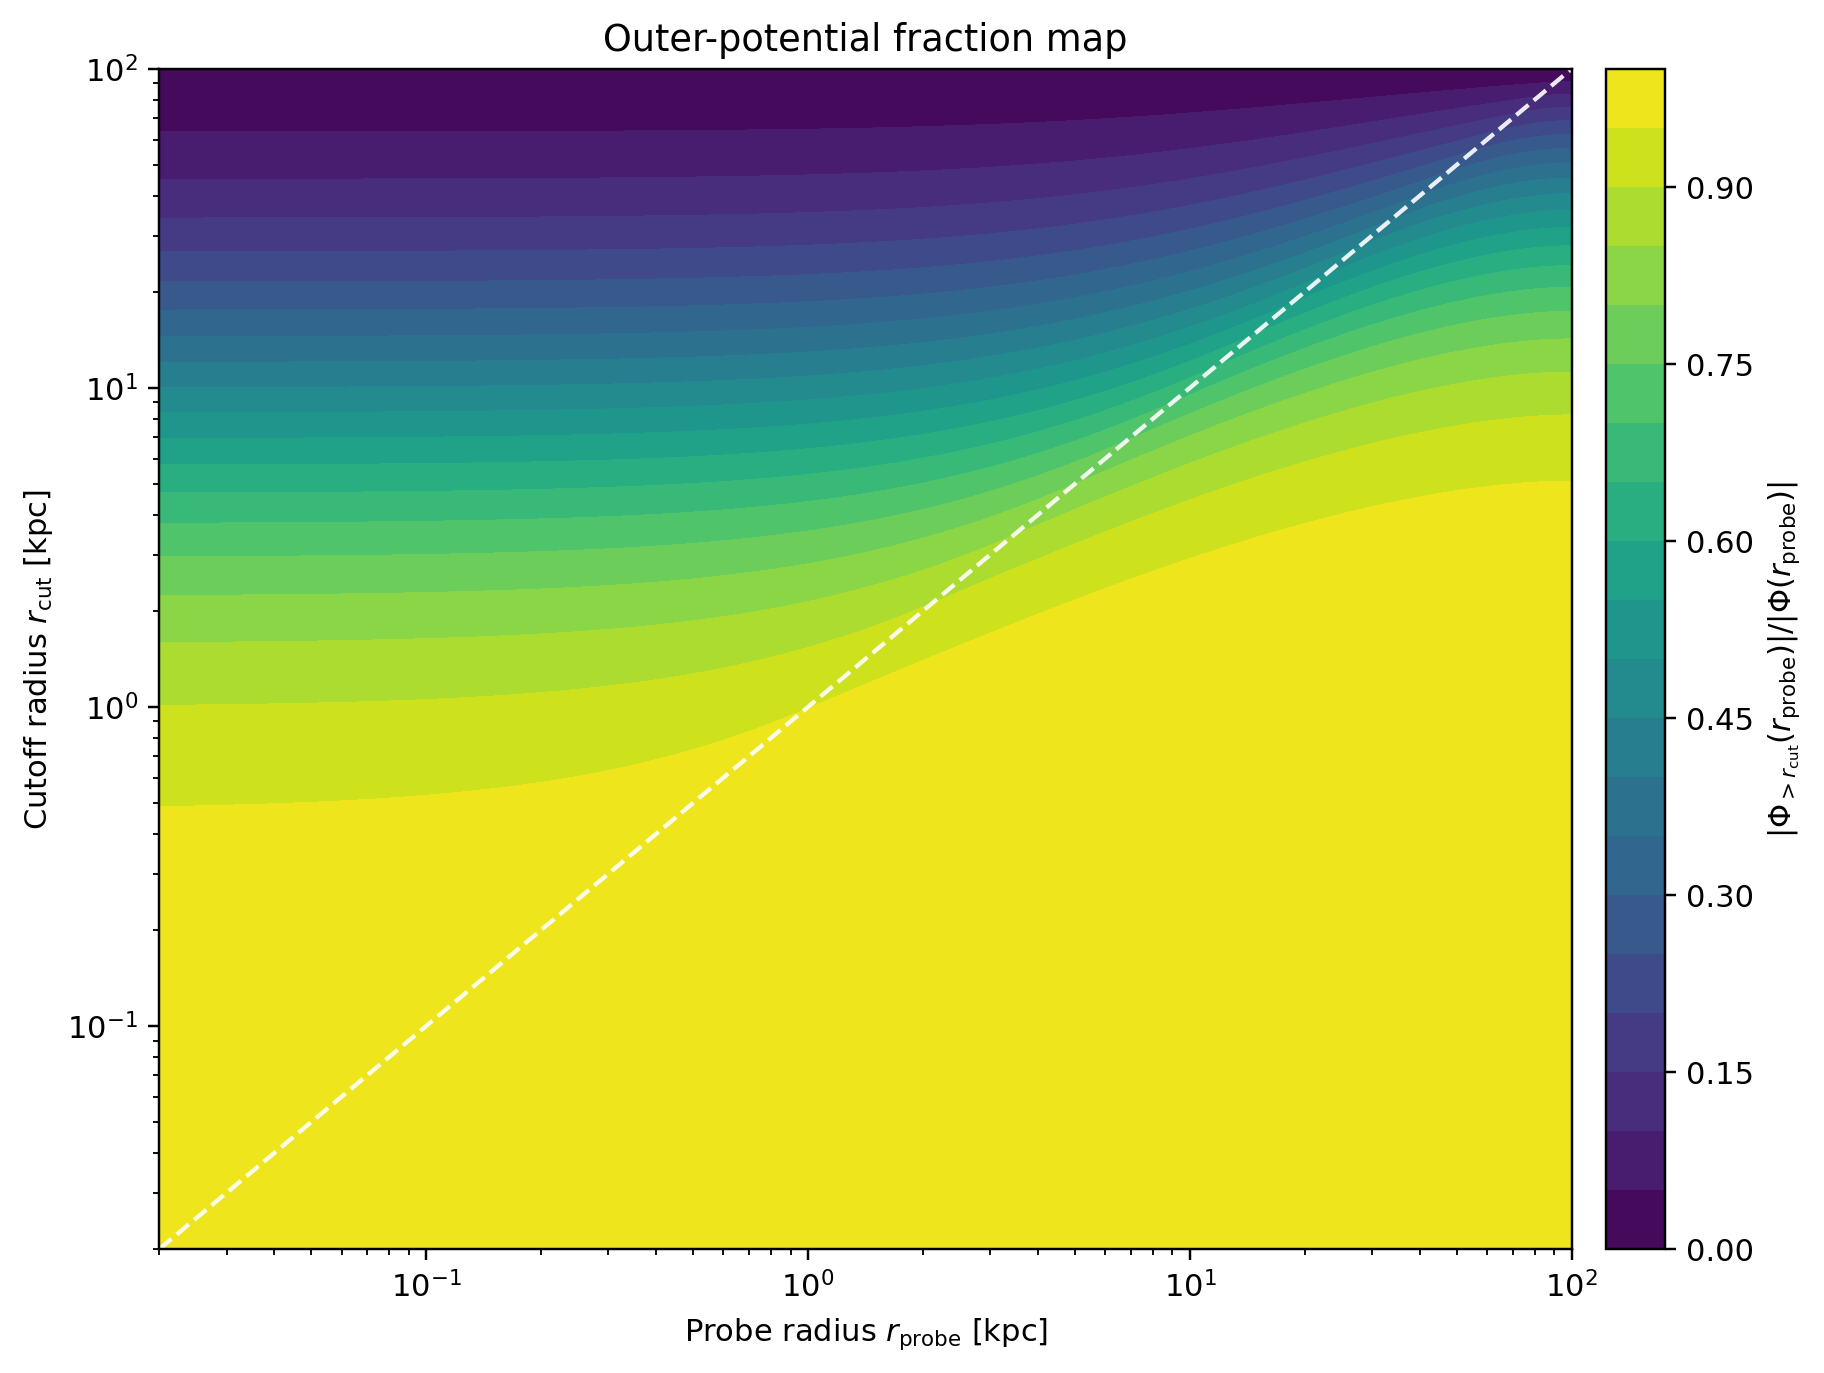
\includegraphics[width=0.85\textwidth]{content/ch5/img/04_outer_fraction_map.png}
	\caption{\textbf{2D map of the outer-potential fraction.} Rows represent probe radii; columns represent cutoff radii. The color intensity indicates the fraction of potential at a given probe radius arising from material beyond the cutoff. The transition from high (red) to low (blue) values shows the radius beyond which the outer halo becomes a small correction.}
	\label{fig:results_shell_map}
\end{figure}

The 2D map reveals the structure clearly: for small cutoff radii (lower rows), a broad range of inner probe radii feel substantial outer halo influence. As the cutoff moves outward, this influence shrinks to a narrow band near the cutoff itself.

\subsection{Interpretation and implications}

The analytic shell study establishes that the outer halo is not dynamically negligible, it contributes substantially to the potential structure experienced by inner particles, even if it does not directly modify the local force field. This has two important consequences:

\begin{enumerate}
\item \textbf{Motivation for the hybrid model}: A simulation in which the inner region ($r < r_{\mathrm{cut}}$) evolves with particles while the outer region ($r > r_{\mathrm{cut}}$) is represented by an analytic potential can only reproduce the true inner evolution if the outer potential is represented accurately.

\item \textbf{Tests of shell-coupling mechanisms}: If the persistent central density decline arises from global halo coupling, where the outer shells modulate the potential experienced by inner particles, then a hybrid model should produce a noticeably different evolution. Conversely, if the decline persists even in the hybrid setup, the mechanism is either purely inner-region dynamics or depends on structures (e.g., substructure, asymmetries) not captured by a smooth analytic outer potential.
\end{enumerate}

Therefore, an outer halo potential that accurately matches the mass distribution should preserve roughly 5--10\% of the outer-potential contribution at the cutoff radius. Whether this degree of fidelity is sufficient to maintain the observed central-density decline, or whether further structural complexity is required, is addressed by the hybrid-model simulations discussed in the next section.
